%!TEX TS-program = Arara
% arara: pdflatex: {shell: yes}
\documentclass[12pt,ngerman]{beamer}

\usepackage[T1]{fontenc}
\usepackage{booktabs}
\usepackage{babel}
\usepackage{graphicx}
\usepackage{csquotes}
\usepackage{xcolor}
\usetheme{metropolis}

\title{Git \& Github nutzen}
\author{Dr. Uwe Ziegenhagen}
\subtitle{\url{github.com/UweZiegenhagen/Github_nutzen}}

\begin{document}

\begin{frame}

\maketitle

\end{frame}

\begin{frame}

\tableofcontents

\end{frame}

\section{Warum?}

\begin{frame}[allowframebreaks]
\frametitle{Einige Zitate (Quelle Google)}

\begin{itemize}
	\item \enquote{Student Tim (26) kommt es vor wie ein schlechter
Traum: Ein kurzer Blackout beim Einkaufen und seine
Laptoptasche ist weg. Darin steckt das Notebook mit der
auf 45 Seiten gespeicherten Abschlussarbeit [...].}
	\item \enquote{Ich bin so verzweifelt und hoffe ihr könnt mir
weiterhelfen. ich bin im zweiten Versuch meiner
Bachelorarbeit und zwei Tage vor Abgabe wird mir mein
Laptop geklaut. Habe leider nur eine nicht fertige Version
meiner Arbeit von paar Wochen auf meinen Stick. werde
ich jetzt exmatrikuliert}
	\item \enquote{Lieber Dieb, meinen Laptop kannst du behalten, aber
bitte schick mir doch die Bachelorarbeit.}

\item \enquote{Natürlich war ich blöd, die Arbeit nicht noch mehr zu
sichern. Aber ich hatte sie ja sogar auf einem USB-Stick
gespeichert [...] Aber der Stick war leider auch in dem
Rucksack mit dem Laptop.}
\item  \enquote{I walk her through letting me remote into her computer,
and she tells me what happened. She stored her thesis on
1 flash drive and that’s it. No backup copies, no syncing
files to the cloud, nothing. Her entire thesis was on a
flash drive. And she lost it.}
\end{itemize}

\end{frame}

\begin{frame}
\frametitle{Grundlegendes}

Für Backups gilt:

\begin{itemize}
\item Backups nicht nur auf dem Gerät lagern!
\item Backups nicht in physischer Nähe lagern!
\item Backup bringt nichts, wenn das Backup nicht zurückgespielt werden kann!
\item Es ist oft sinnvoll, wenn man auf ältere Versionen zurückgreifen kann
\item Ideal: Backup auf anderem Betriebssystem außerhalb der
eigenen Wohnung
\end{itemize}

Lösung: Versionsverwaltungsprogramme, Backup erhält man
als „Nebenprodukt“

\end{frame}

\section{Was?}

\begin{frame}
\frametitle{Geschichtliches}

Wikipedia: \enquote{Eine Versionsverwaltung ist ein System, das zur
Erfassung von Änderungen an Dokumenten oder Dateien
verwendet wird. Alle Versionen werden in einem Archiv mit
Zeitstempel und Benutzerkennung gesichert und können später
wiederhergestellt werden. Versionsverwaltungssysteme werden
typischerweise in der Softwareentwicklung eingesetzt, um
Quelltexte zu verwalten.}

\begin{itemize}
\item SCCS „Source Code Control System“, 1972 in den Bell Labs
\item  RCS, Anfang der 1980er, verwaltet einzelne Dateien
\item  CVS, 1989, Weiterentwicklung von SCCS und RCS
\item  SVN „Subversion“, seit 2000, Apache-Projekt
\item  git, seit 2005, Ersatz für Bitkeeper, Linux Torvalds
\end{itemize}
\end{frame}

\begin{frame}
\frametitle{Zentral oder dezentral}

{\bfseries Zentraler Ansatz bei SVN}

\begin{itemize}
	\item zentraler Server, Clients holen sich die Daten
	\item Nutzer bearbeiten den Code
	\item nach der Arbeit: Code wieder auf den Server
	\item habe ich persönlich lange auf meinem Synology NAS genutzt
\end{itemize}

{\bfseries Dezentraler Ansatz bei git}

\begin{itemize}
	\item komplexer als SVN
	\item jeder Client hat komplettes Repository mit allen Änderungen
	\item Versionsverwaltung kann komplett offline erfolgen, commits können auf Server gepushed werden
\end{itemize}

\end{frame}

\section{Wie?}

\begin{frame}
\frametitle{Neues Repository anlegen}

\begin{center}
\fbox{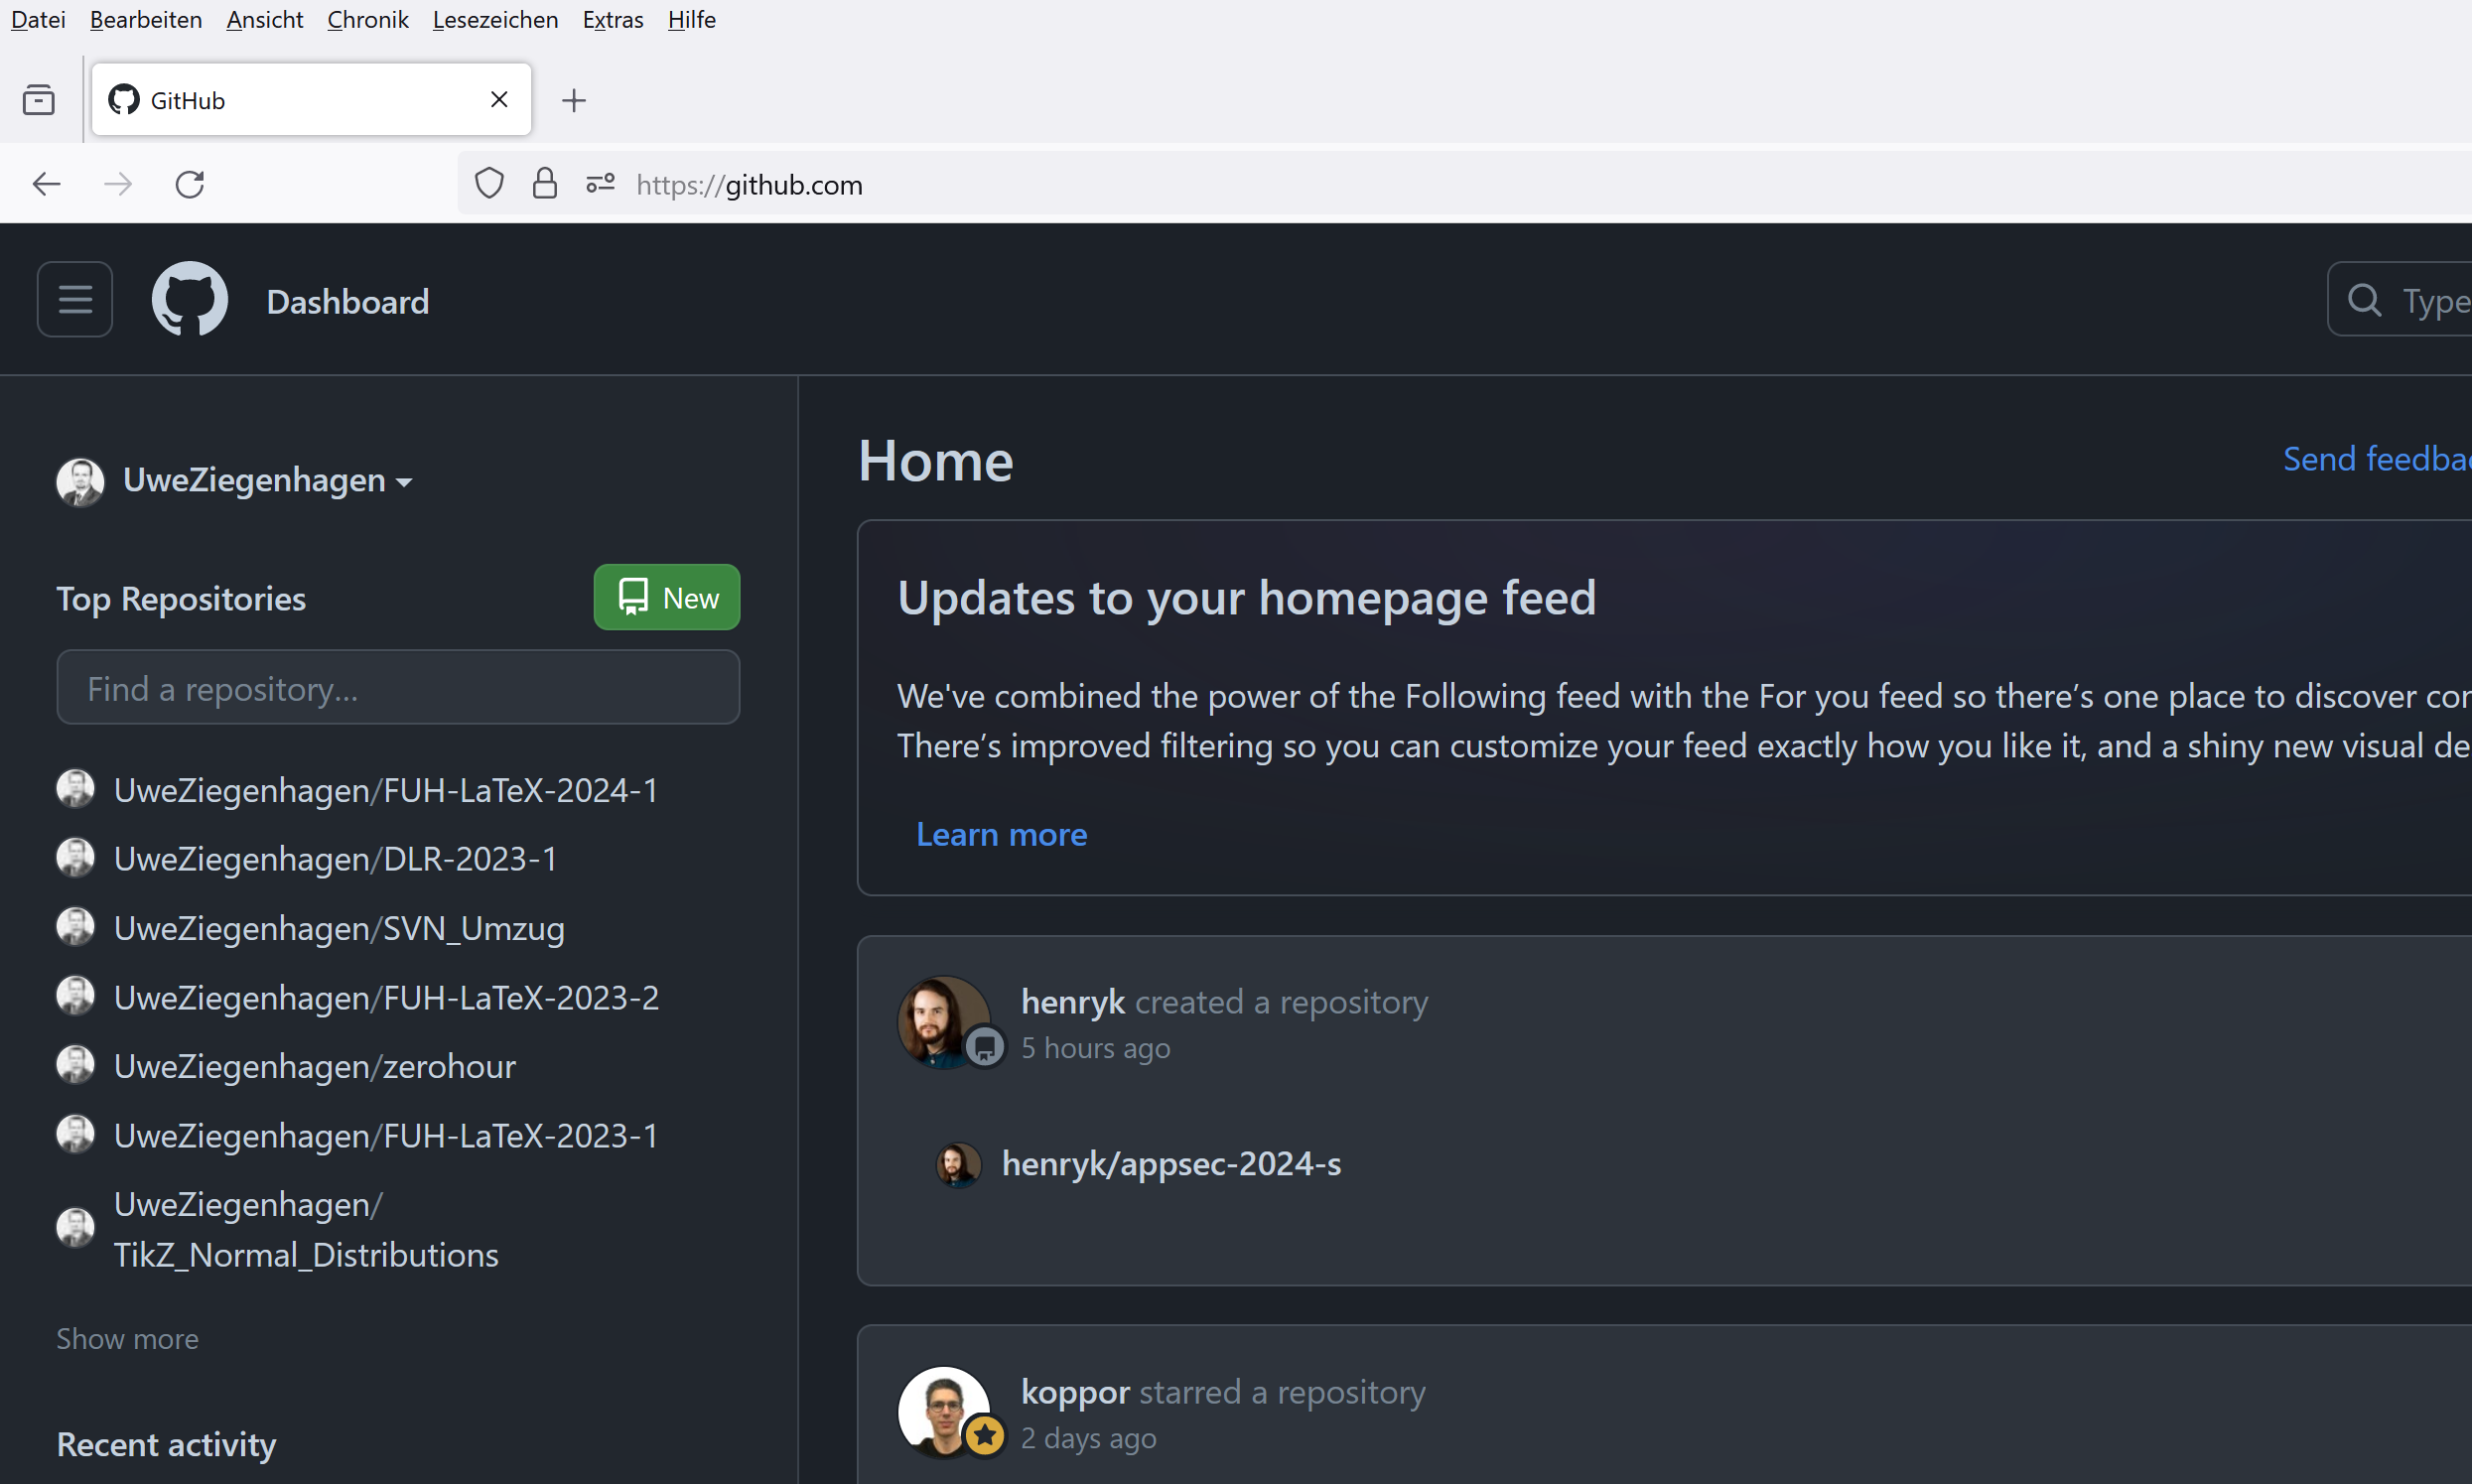
\includegraphics[width=0.95\textwidth]{Bilder/gh-01}}
\end{center}

\end{frame}

\begin{frame}
\frametitle{Public oder Private?}

\begin{center}
\fbox{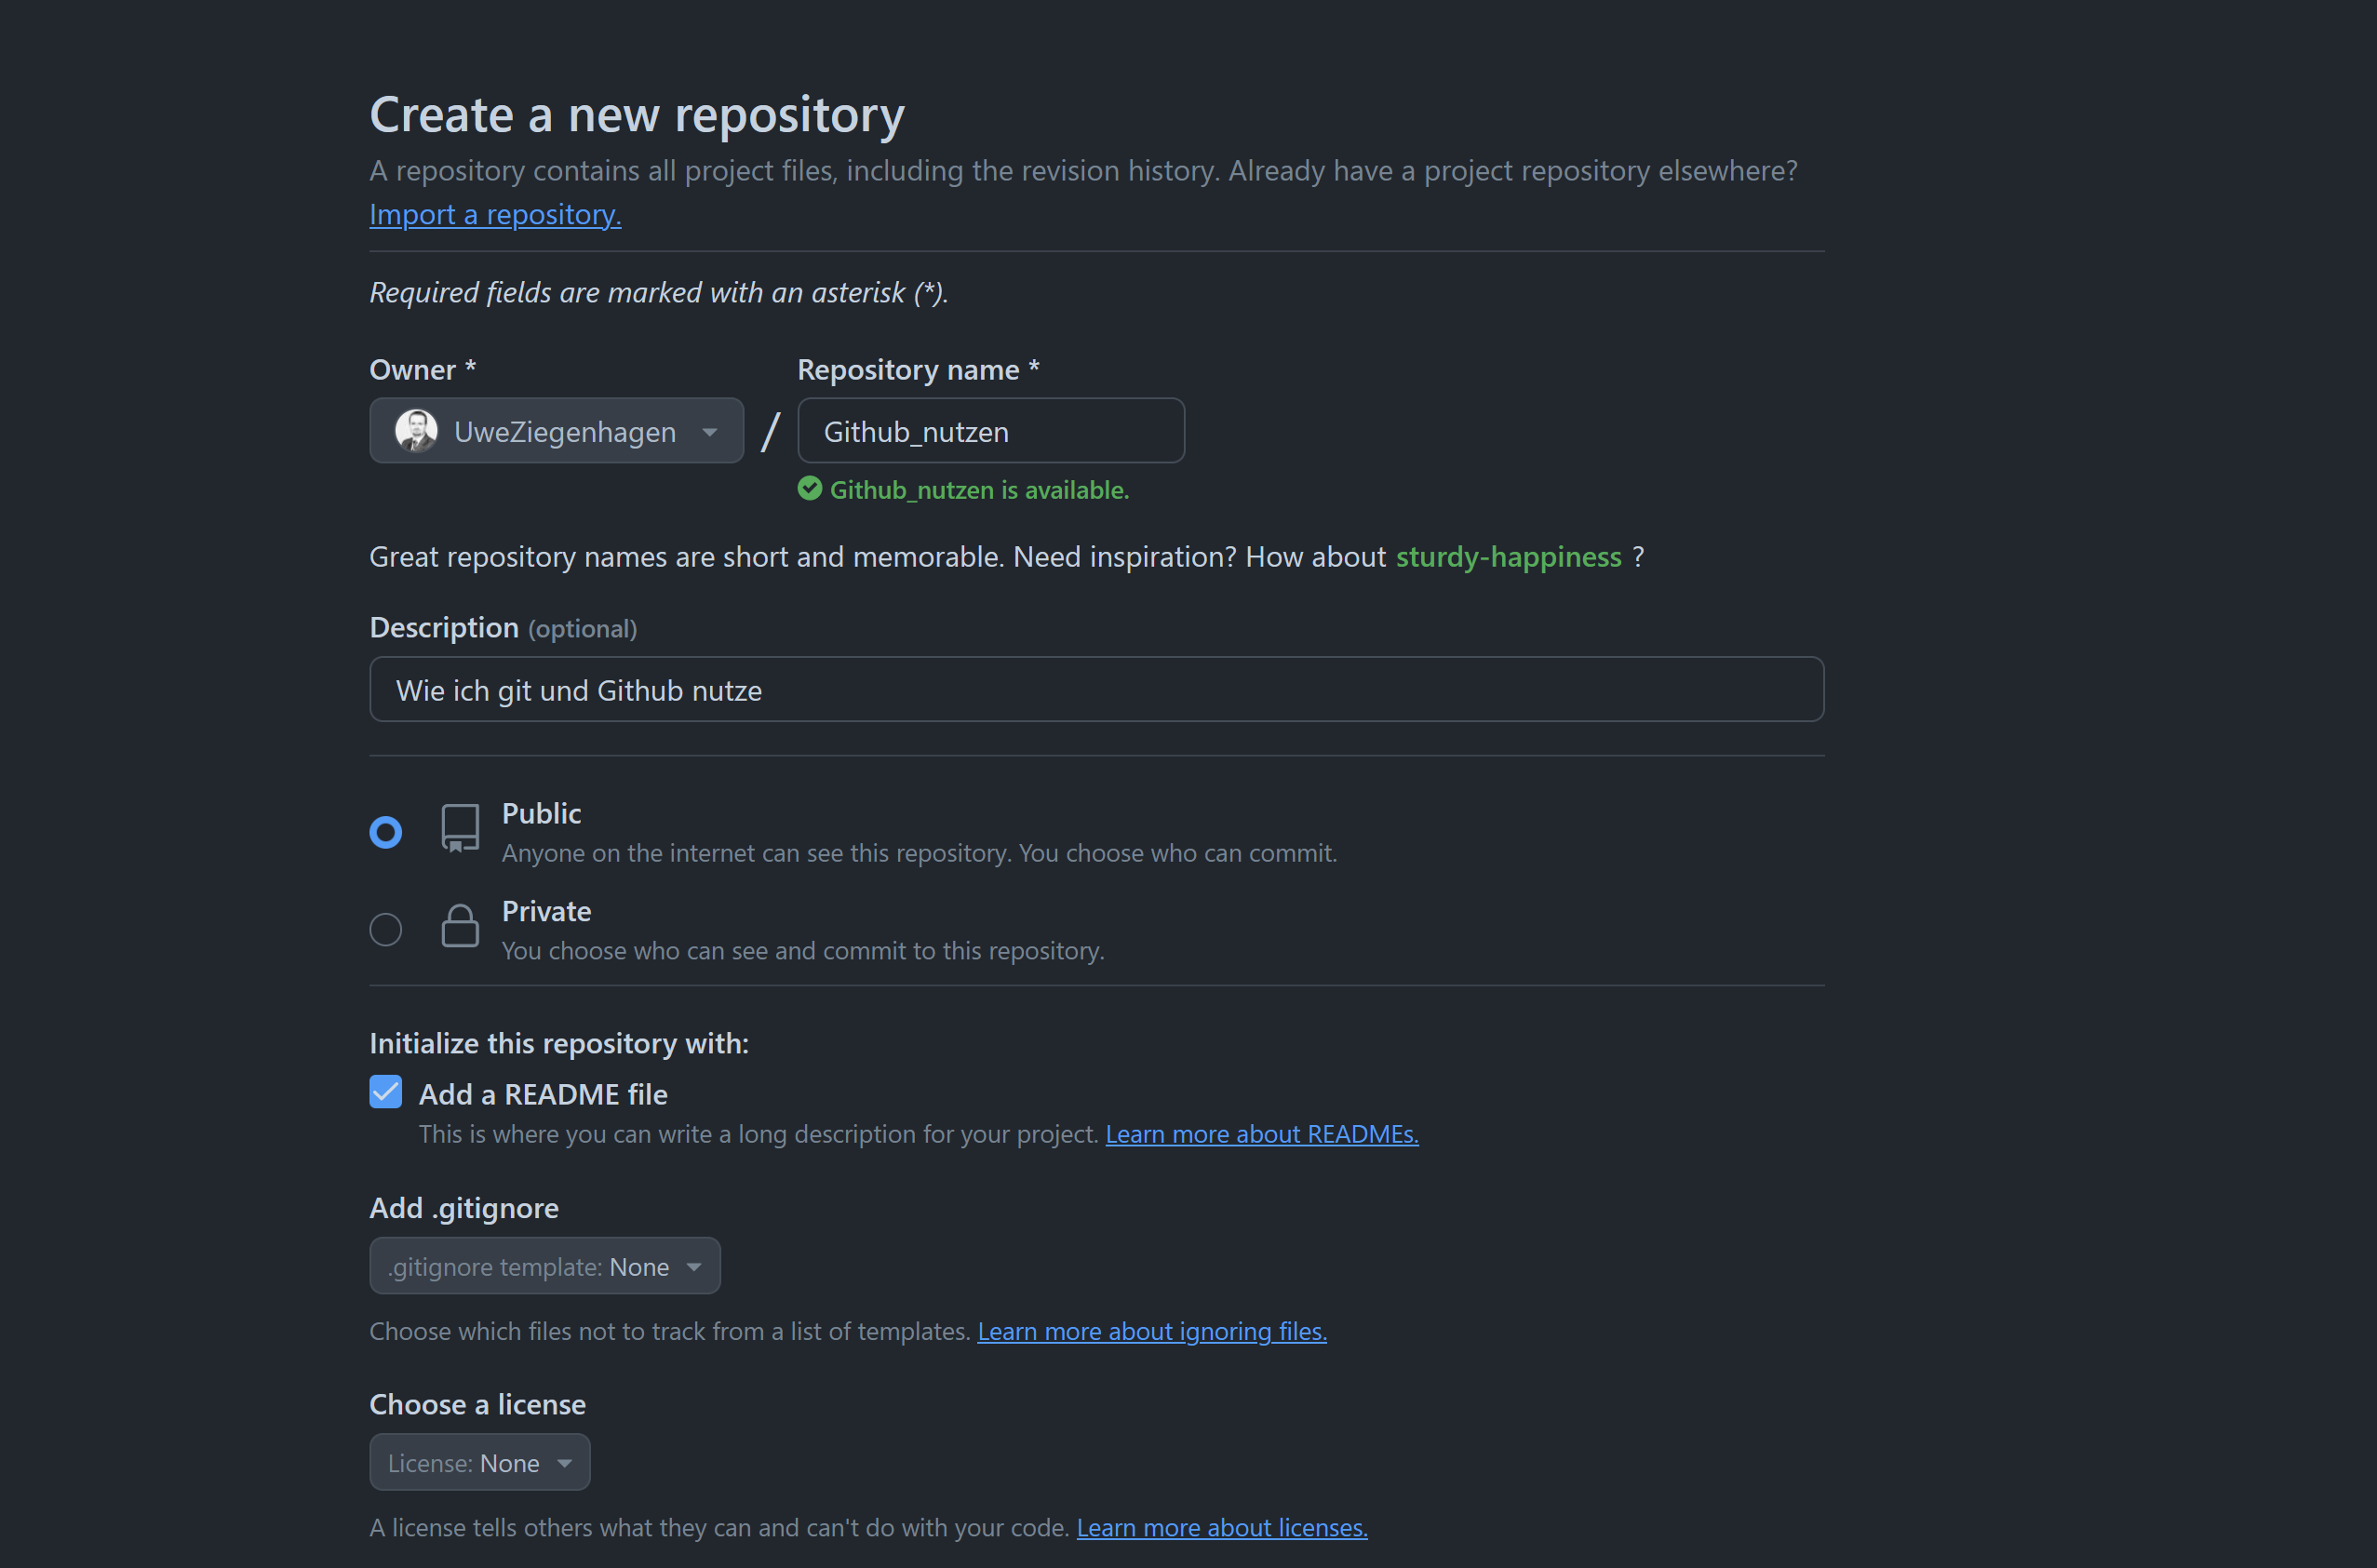
\includegraphics[width=0.95\textwidth]{Bilder/gh-02}}
\end{center}

\end{frame}

\begin{frame}
\frametitle{URL kopieren}

\begin{center}
\fbox{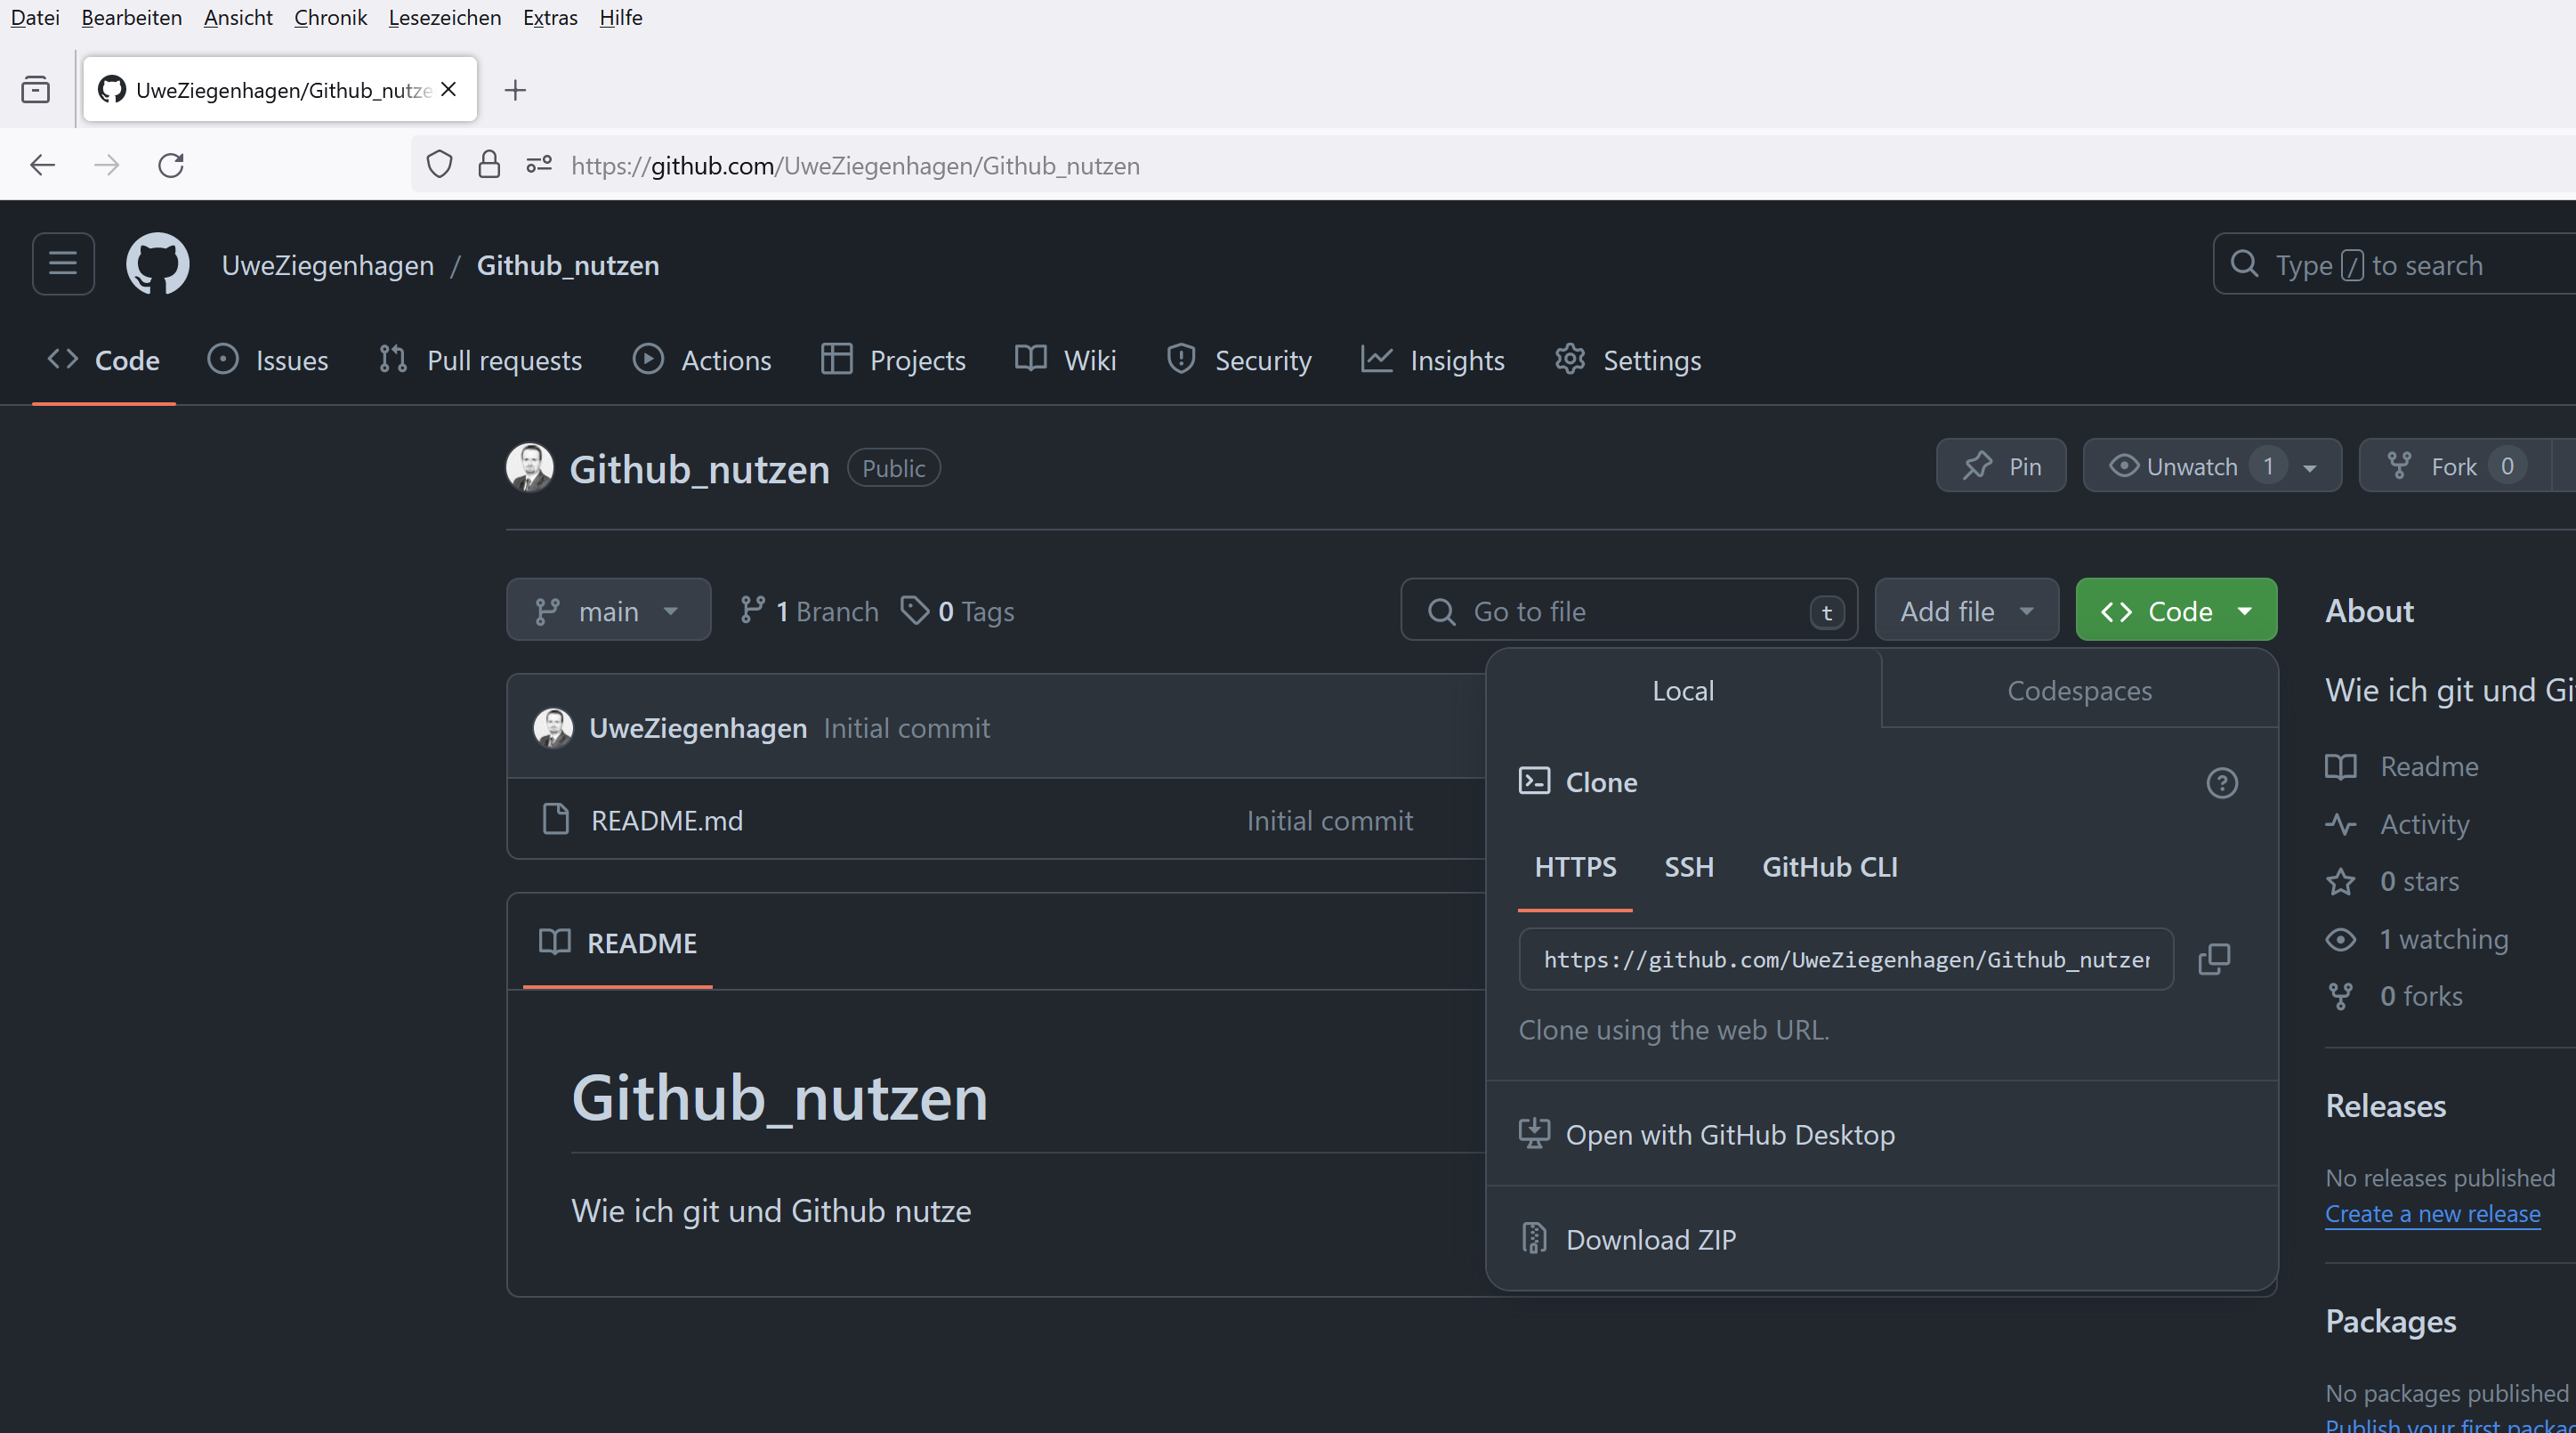
\includegraphics[width=0.95\textwidth]{Bilder/gh-03}}
\end{center}

\end{frame}

\begin{frame}
\frametitle{In Github Desktop klonen I}

\begin{center}
\fbox{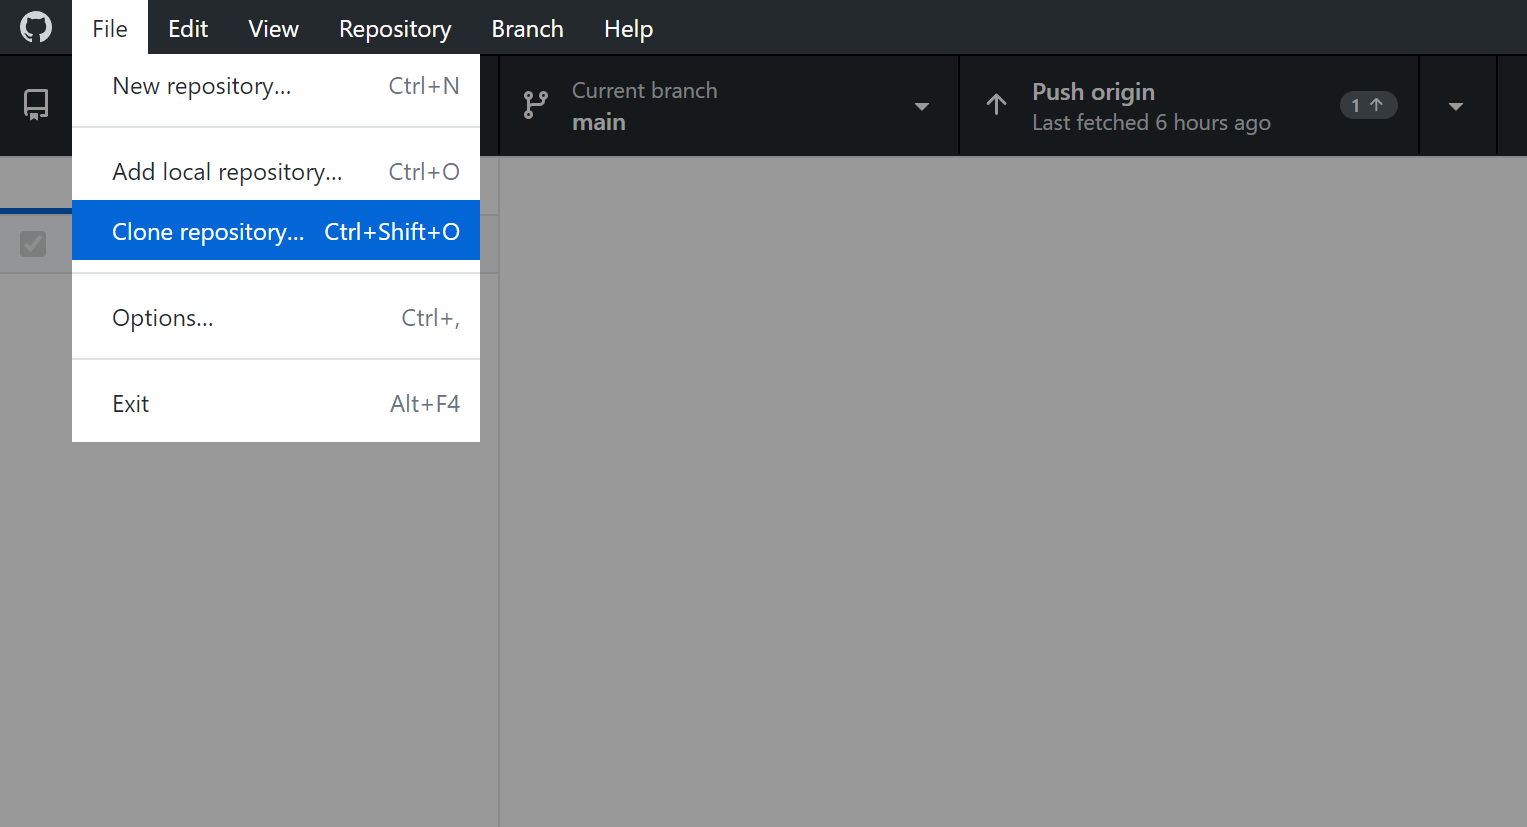
\includegraphics[width=0.95\textwidth]{Bilder/gh-04}}
\end{center}

\end{frame}

\begin{frame}
\frametitle{In Github Desktop klonen II}

\begin{center}
\fbox{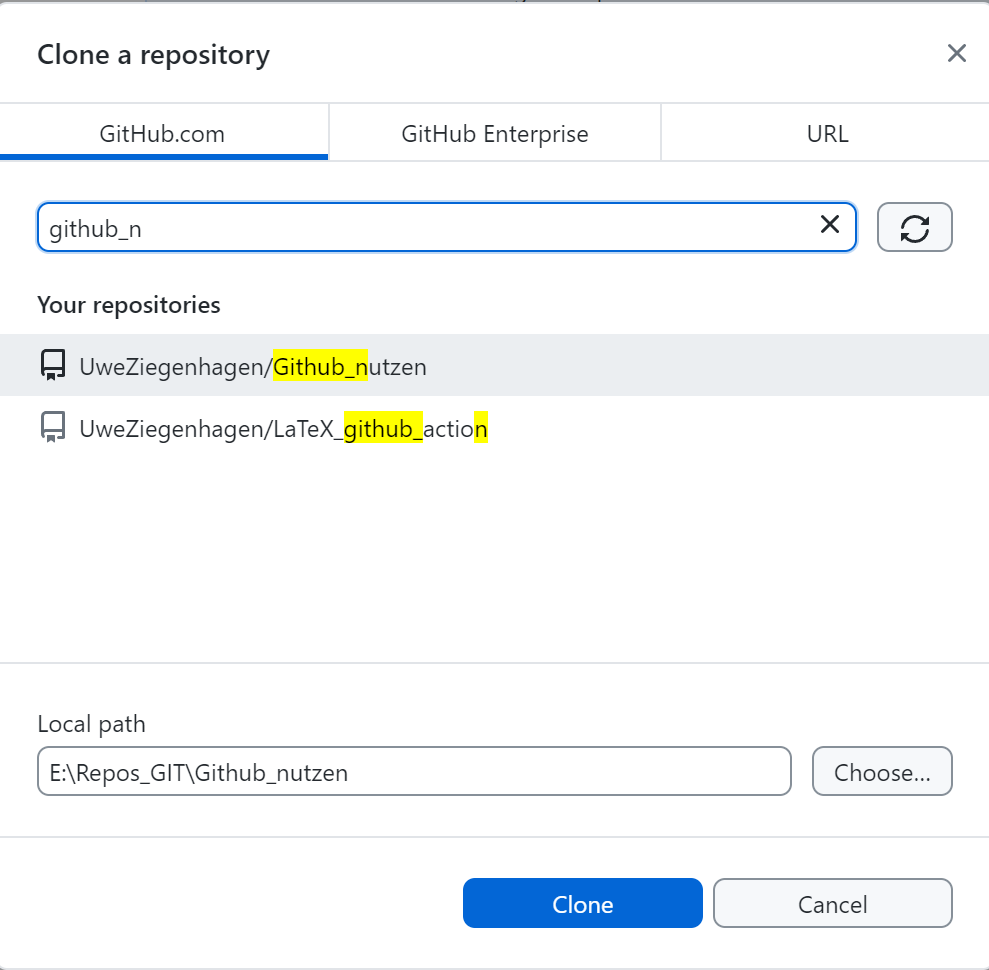
\includegraphics[height=0.85\textheight]{Bilder/gh-05}}
\end{center}

\end{frame}

\begin{frame}
\frametitle{Leeres Repository}

\begin{center}
\fbox{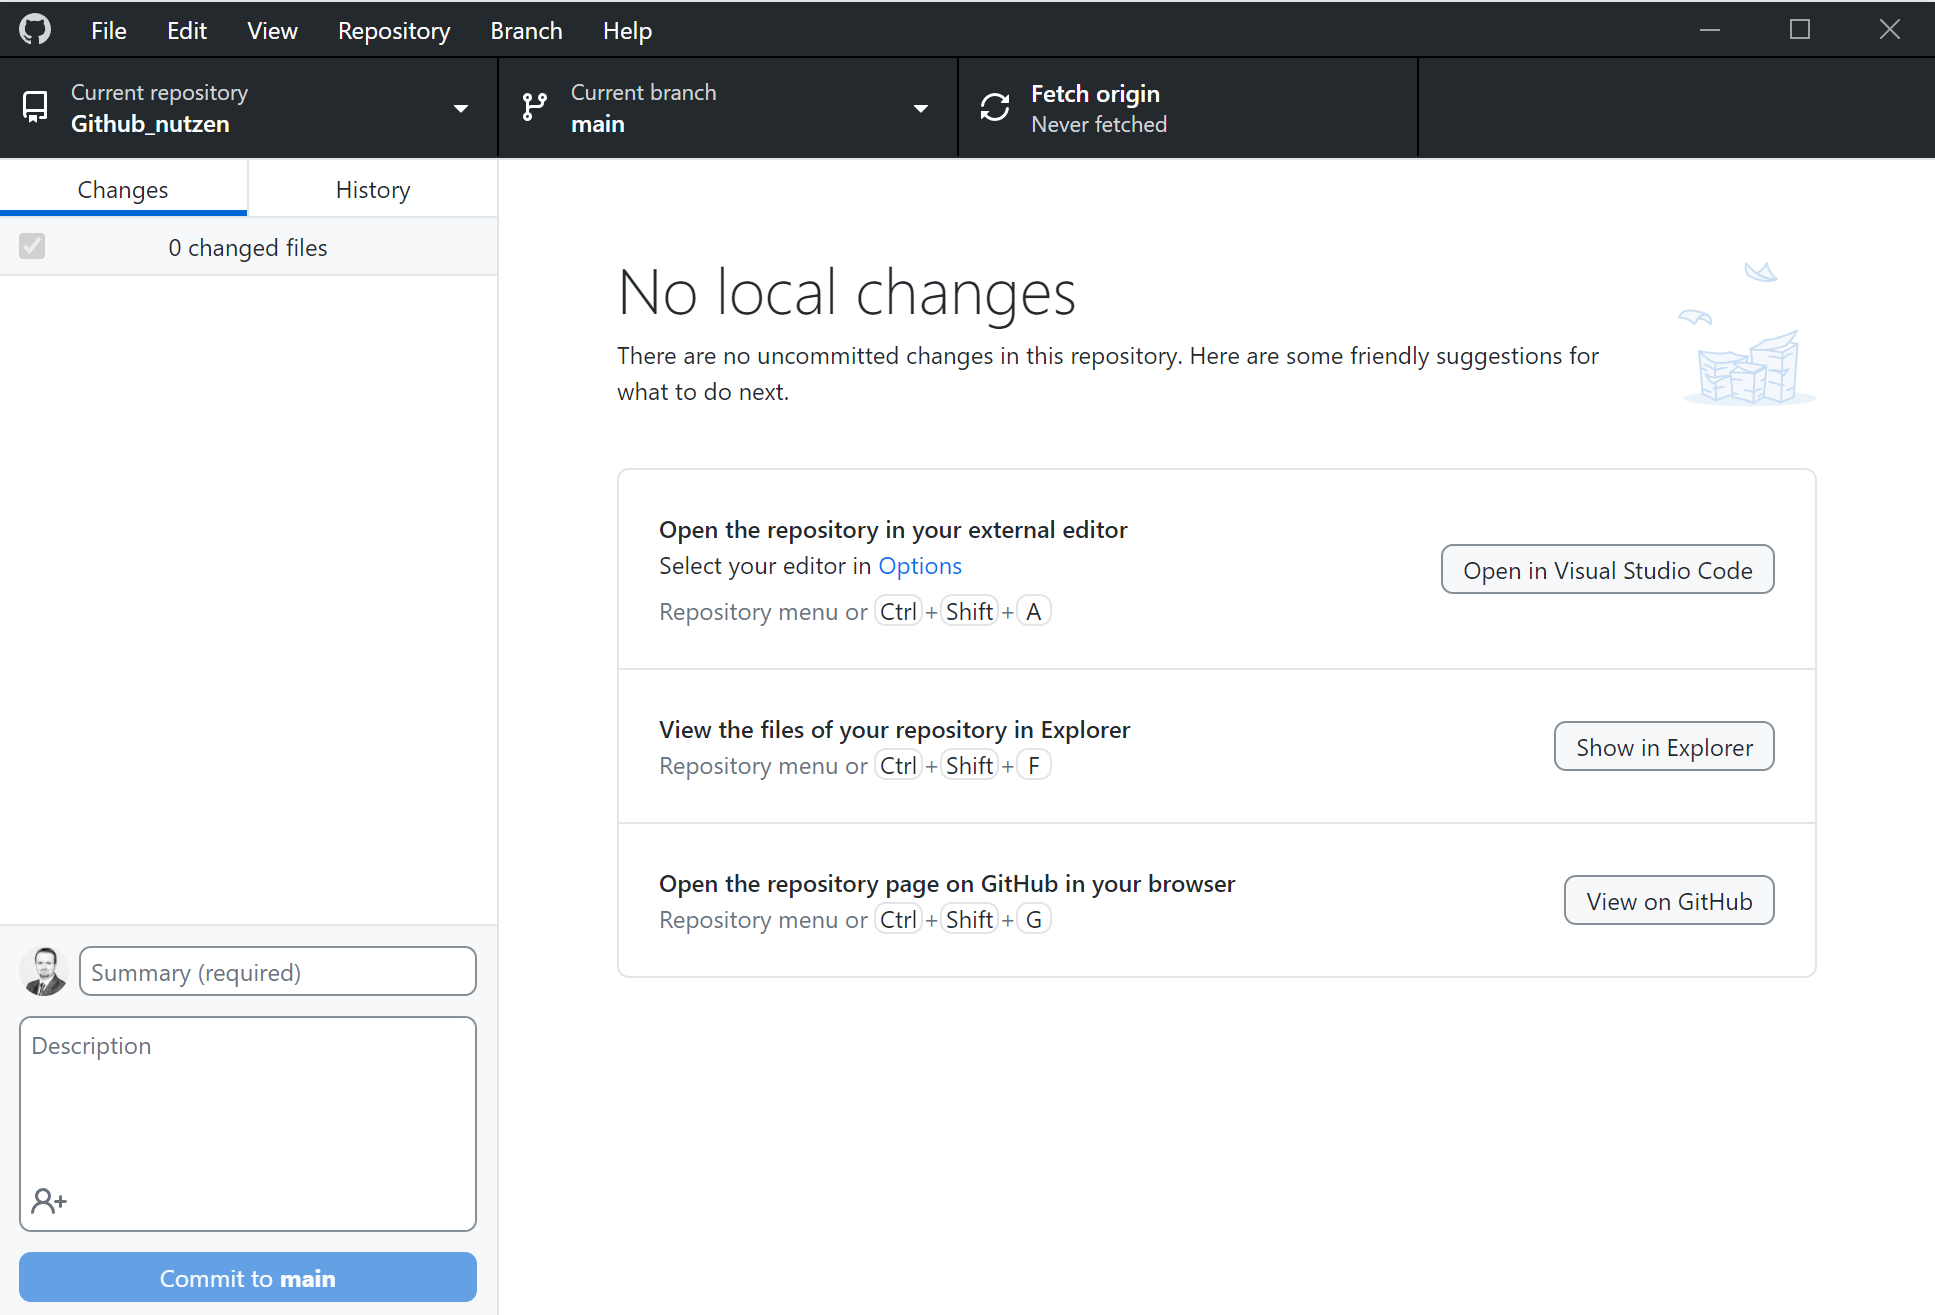
\includegraphics[width=0.75\textwidth]{Bilder/gh-06}}
\end{center}

\end{frame}

\begin{frame}
\frametitle{Arbeiten im Repo}

\begin{center}
\fbox{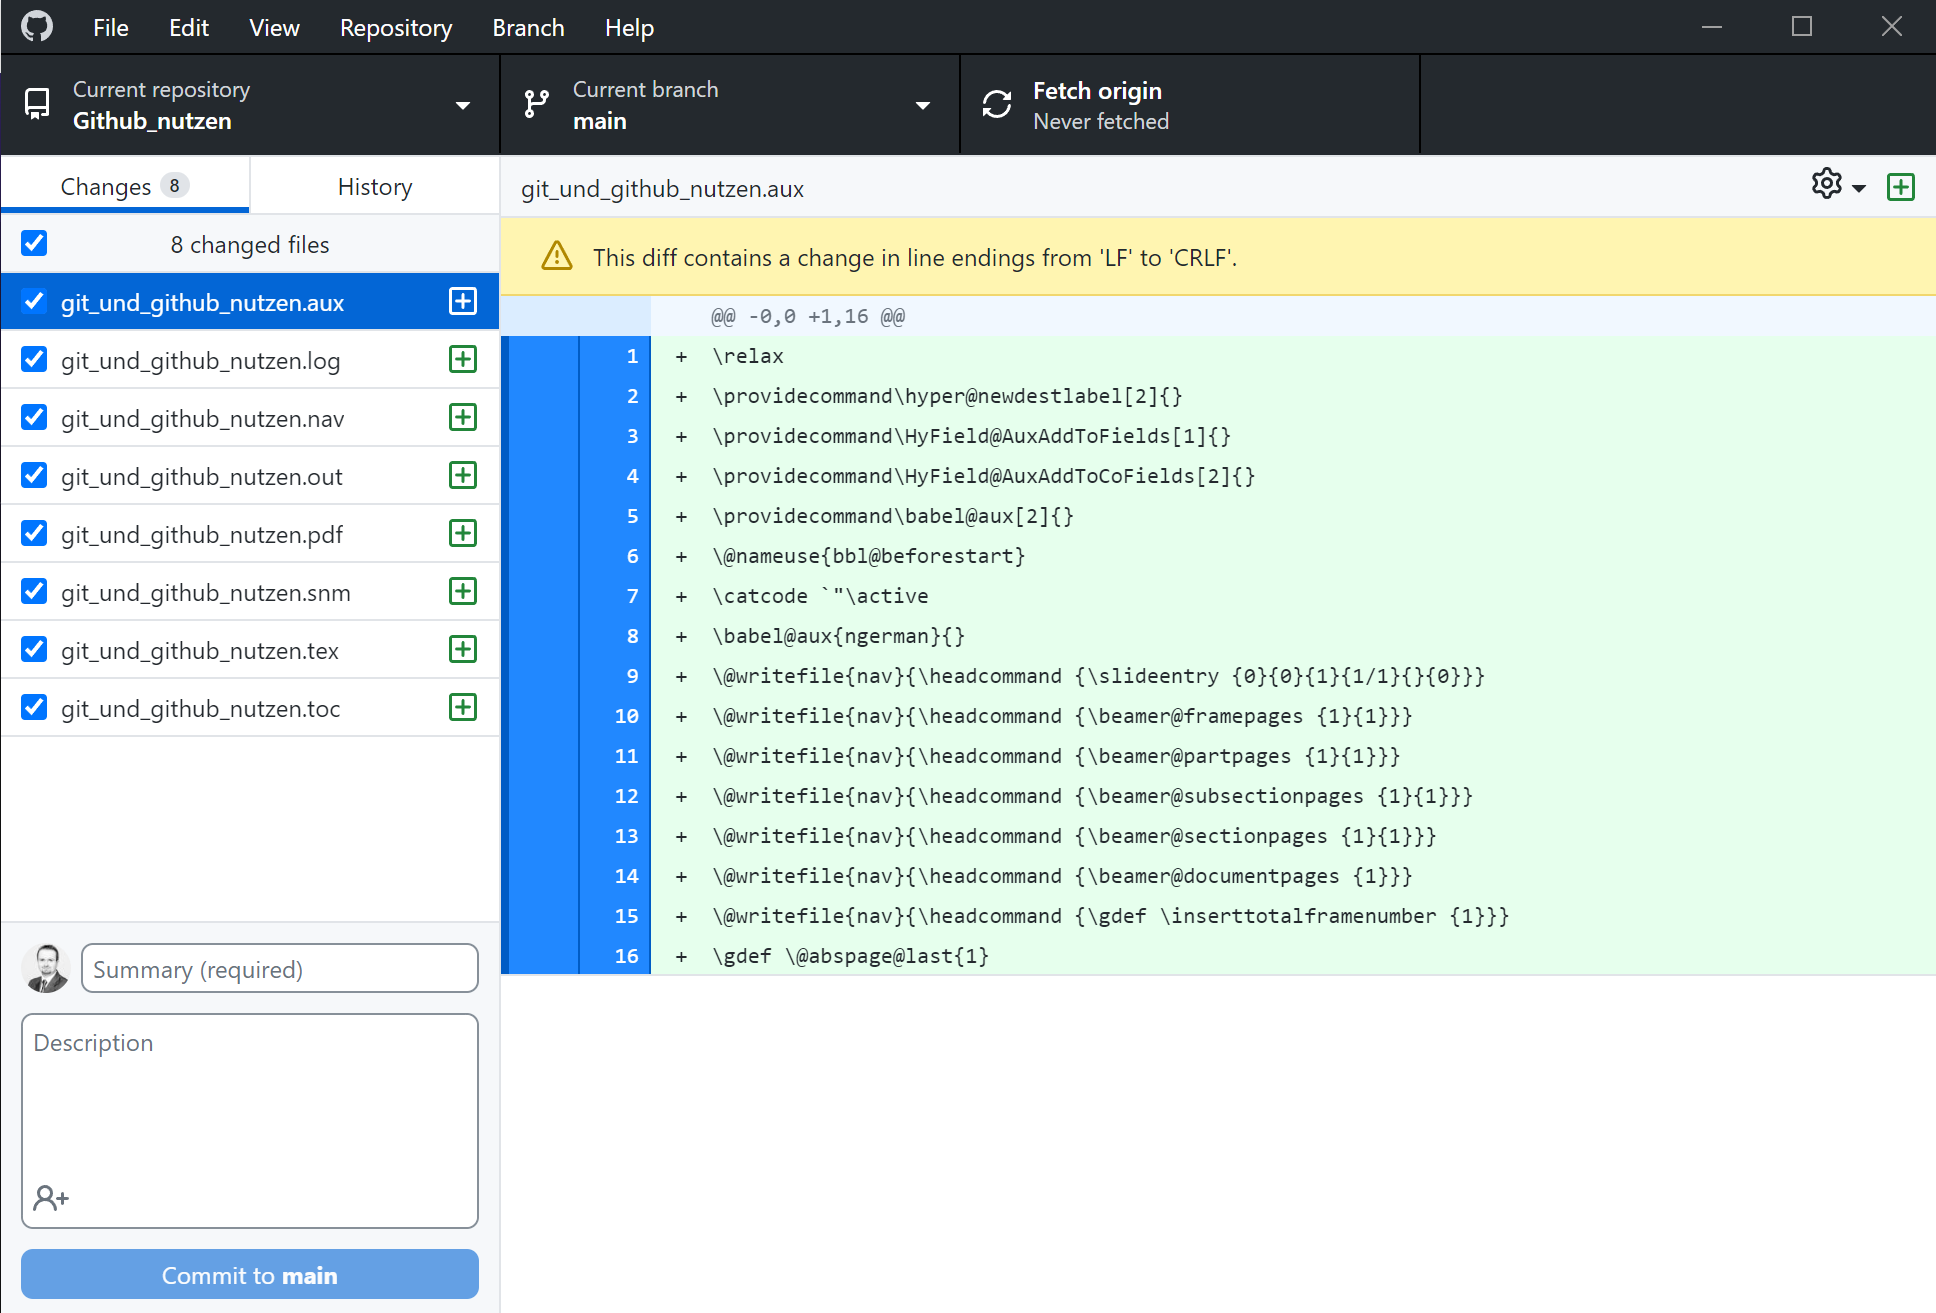
\includegraphics[width=0.95\textwidth]{Bilder/gh-07}}
\end{center}

\end{frame}

\begin{frame}
\frametitle{Unwichtige Dateien for \texttt{.gitignore}}

\begin{center}
\fbox{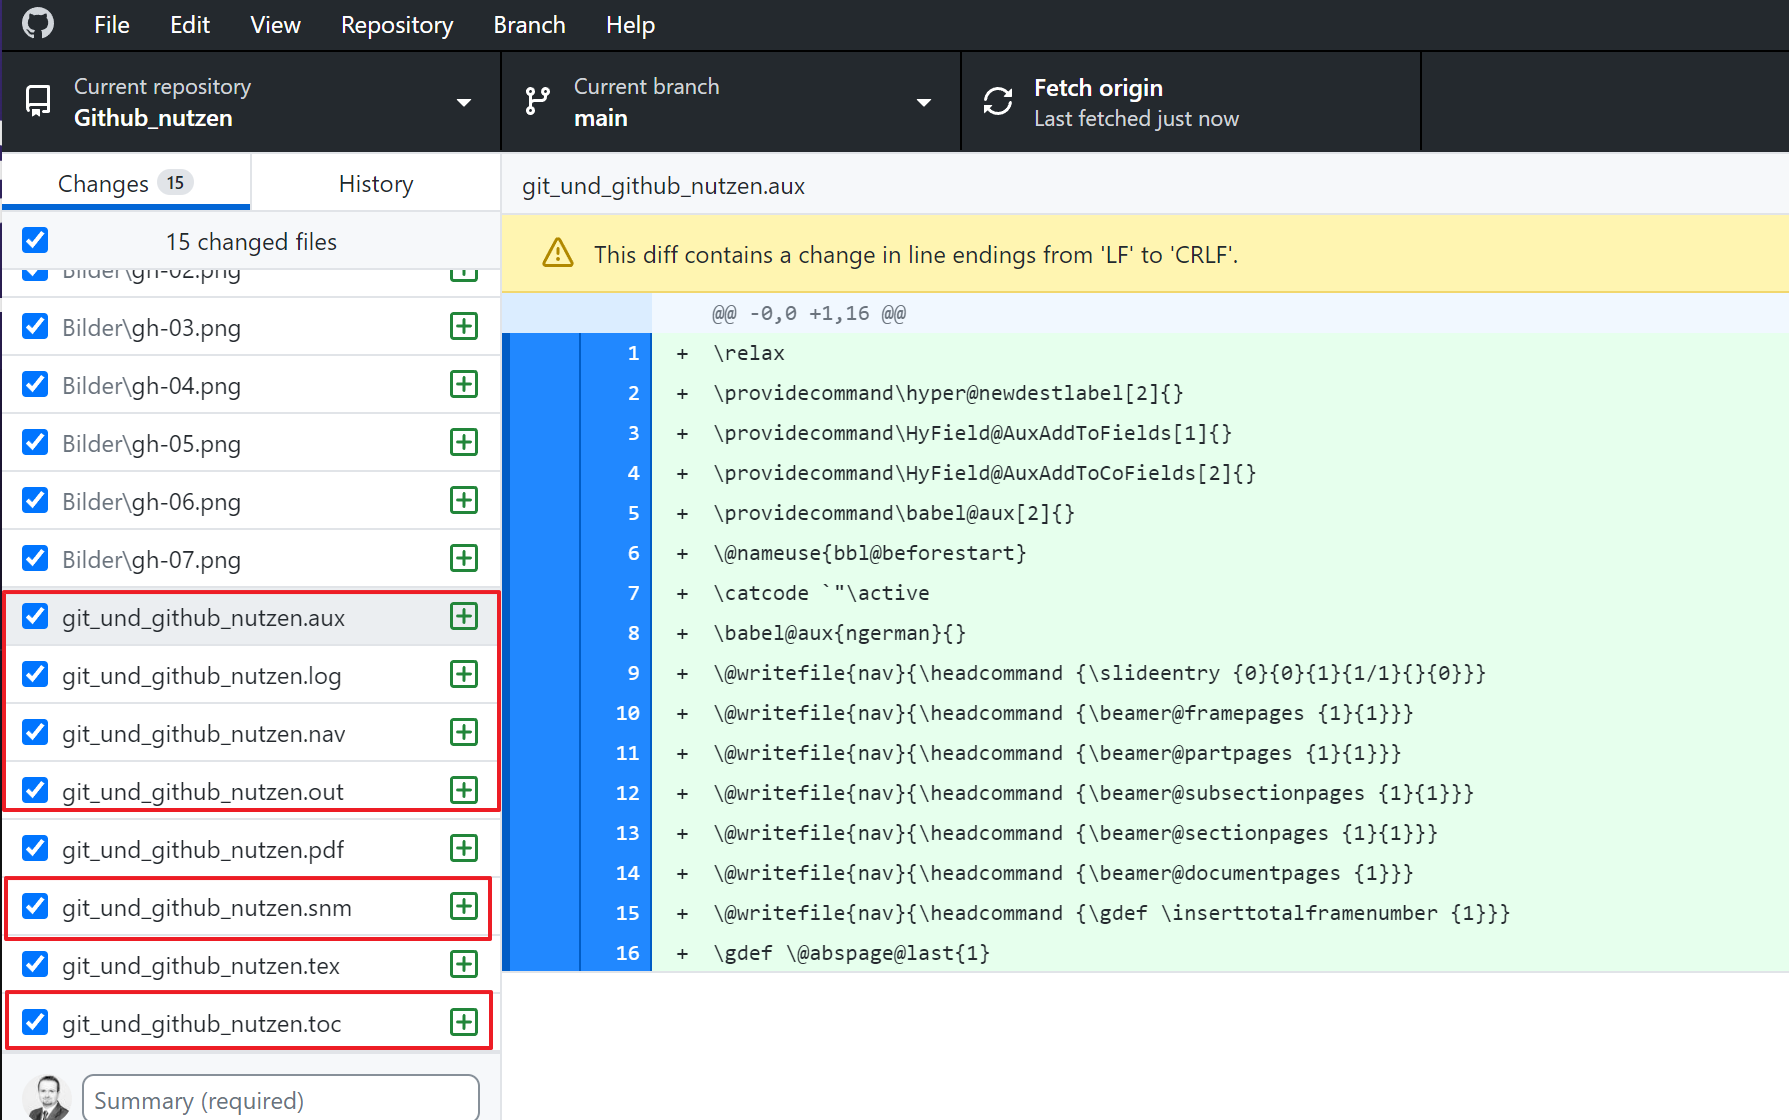
\includegraphics[width=0.95\textwidth]{Bilder/gh-08}}
\end{center}

\end{frame}

\begin{frame}
\frametitle{Push commits to origin}

\begin{center}
\fbox{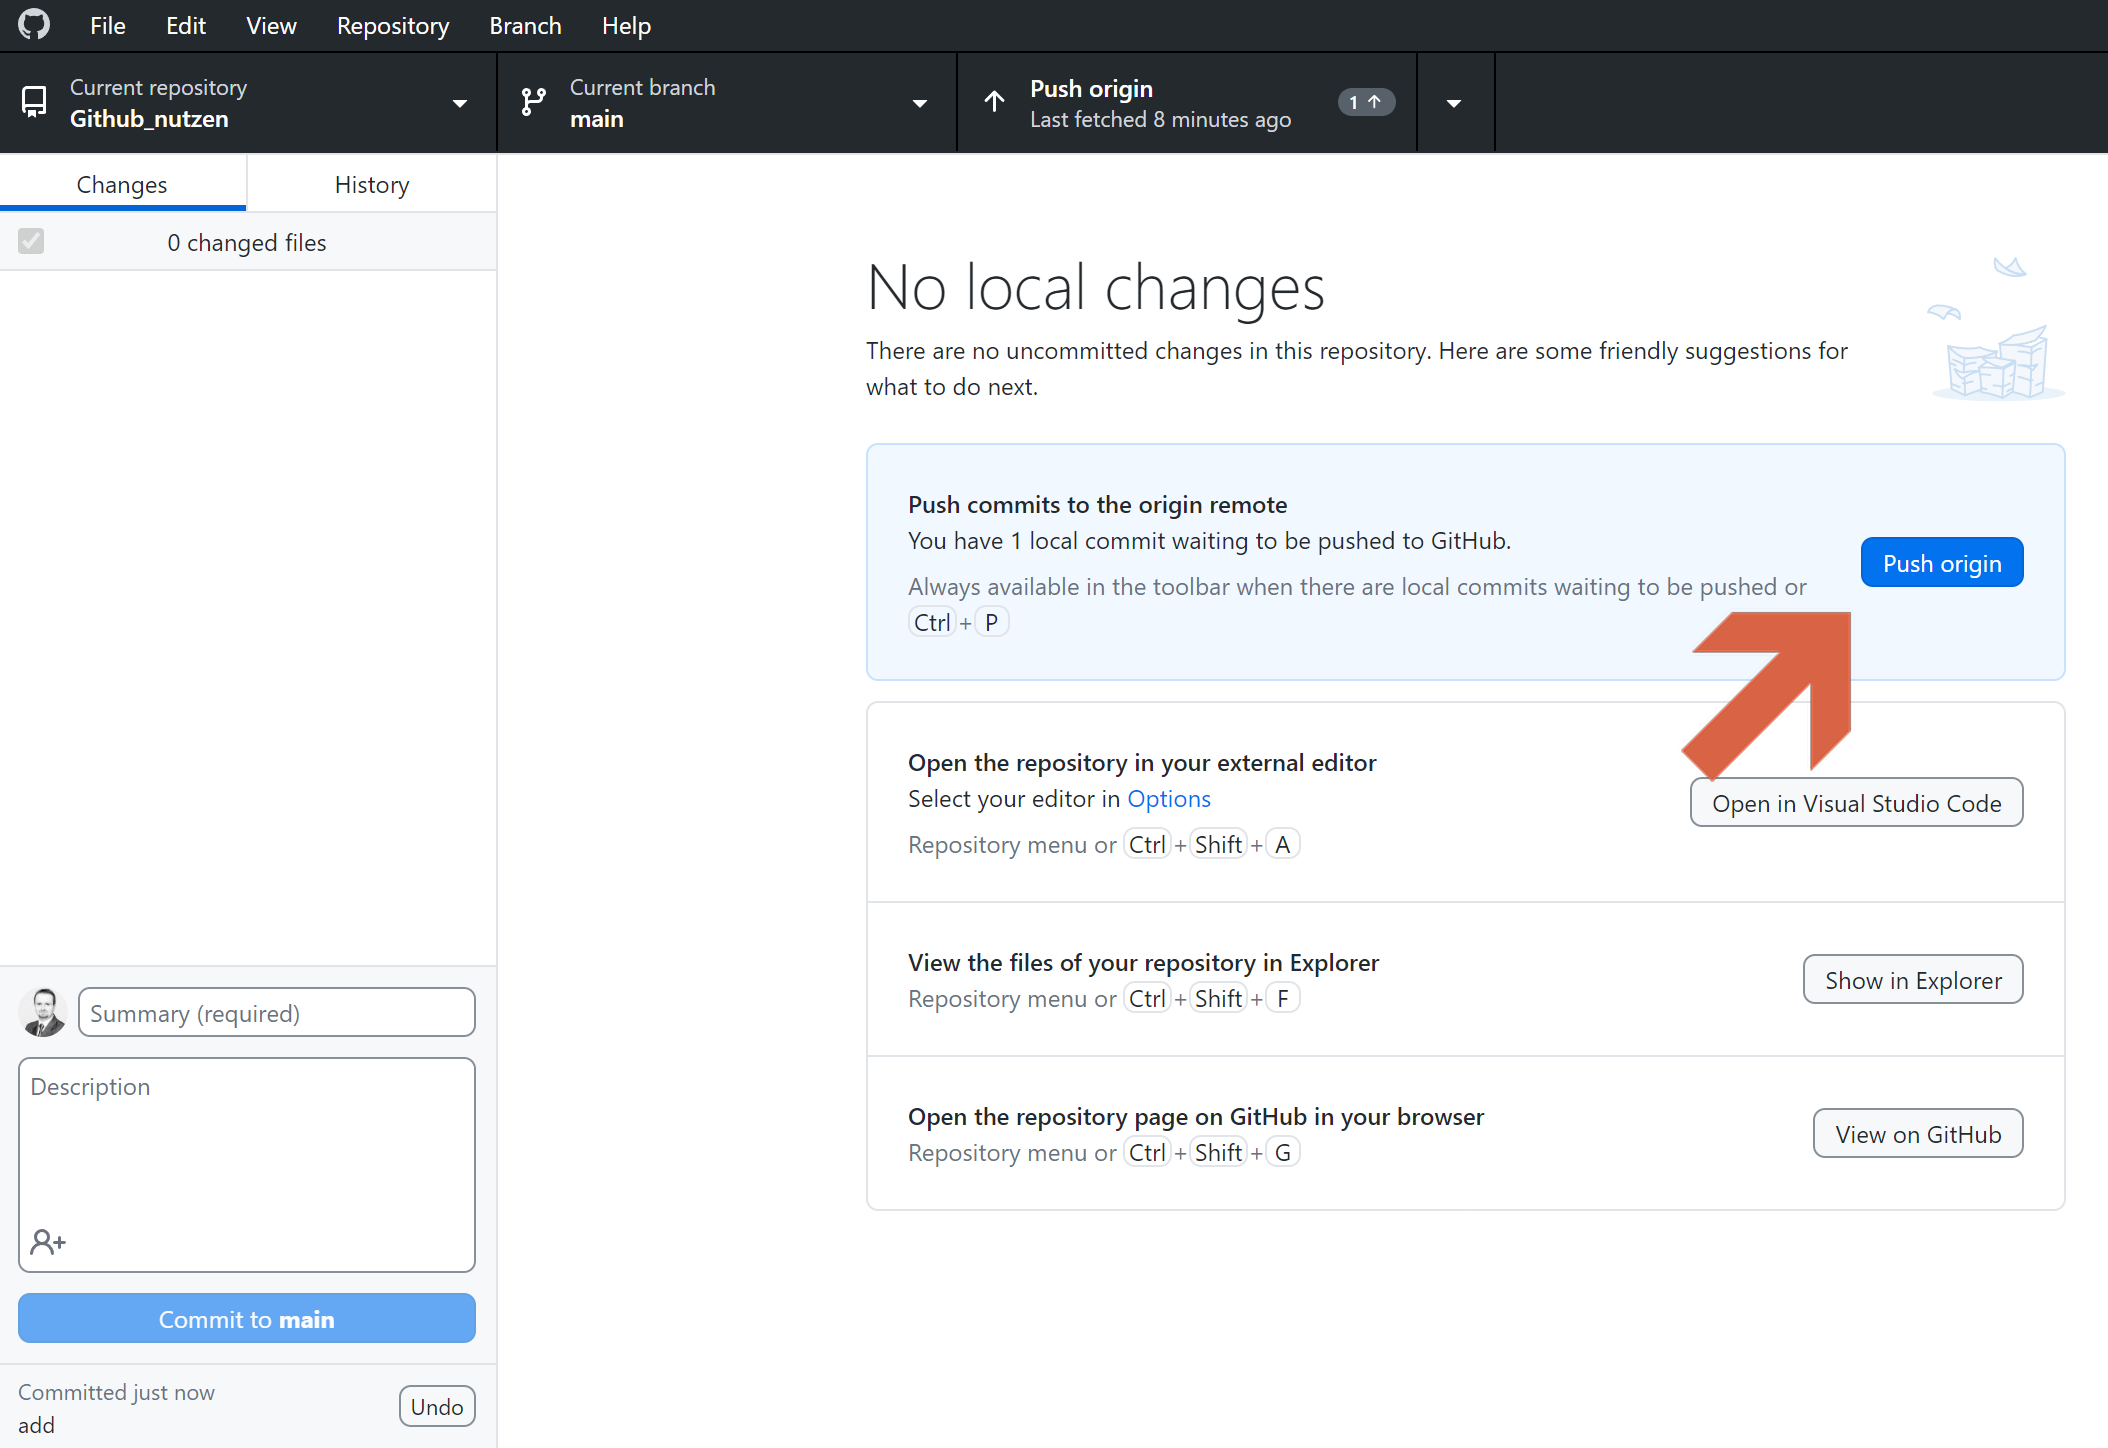
\includegraphics[width=0.95\textwidth]{Bilder/gh-09}}
\end{center}

\end{frame}



\end{document}